\chapter{Design Recursion}\label{chap:recursive_algorithm}
\section{Thinking in Recursion}
{\color{blue}{Recursive algorithms}} are a method of problem solving that involves a function calling itself as a subroutine.
\subsection{Steps to Design Recursive Algorithms}\label{subsec:steps_to_design_recursive_algorithms}
Once a problem is identified as suitable for a recursive approach, the steps to design the recursive algorithm are as follows:
\begin{enumerate}
	\item Define the {\color{blue}{function signature}}, including {\color{blue}{parameters}} and {\color{blue}{return value}}. This often relies on {\color{blue}{experience}}, but sometimes requires a bit of {\color{blue}{creativity}} and {\color{blue}{imagination}}.
	\item Determine the {\color{blue}{base cases}}. These are the simplest instances of the problem, which {\color{blue}{can be solved directly without further recursion}}.
	\item {[Optional]} Determine the {\color{blue}{termination condition of the whole problem}}. This is when the problem is solved, indicating the end of the whole function. It should be noted that sometimes this condition does not exist, e.g., DFS for traversing a graph.
	\item Build the connection between {\color{blue}{larger problem}} and {\color{blue}{smaller sub-problems}}. Ensure that the {\color{blue}{original problem}} can be broken down into {\color{blue}{base cases}}.
\end{enumerate}

\subsection{Recursion and Activation Tree}
{\color{ForestGreen}{It is always beneficial if you can expand a \ul{recursion} as a \ul{activation tree} in your mind.}}\\

By tracking the {\color{blue}{pushes (procedure calls)}} and {\color{blue}{pops (procedure returns)}} of activation records on the call stack, we can save the sequence of activations of the entire program in a {\color{blue}{activation tree}}, which is a good way to illustrate how the call stack works. In this tree, each node corresponds to an {\color{blue}{activation record}}. The steps to establish the activation tree are as follows:
\begin{itemize}
	\item Set the activation of the main procedure as the root node.
	\item When a procedure is called, add a child node to the current node on the right.
	\item When a procedure returns, we move back up to the parent node.
\end{itemize}

This activation tree can then be seen as a comprehensive view of the program's procedural flow:
\begin{itemize}
	\item Each node in the tree corresponds to a {\color{blue}{activation record}}.
	\item The sequence of {\color{blue}{procedure calls}} corresponds to a {\color{blue}{preorder traversal of the activation tree}}.
	\item The sequence of {\color{blue}{procedure returns}} corresponds to a {\color{blue}{postorder traversal of the activation tree}}.
	\item Suppose that control lies within a particular activation of some procedure, corresponding to a node $N$ of the activation tree. Then the activations that are currently active are those that correspond to node $N$ and its ancestors. The order in which these activations were called is the order in which they appear along the path to $N$ , starting at the root, and they will return in the reverse of that order.
\end{itemize}

\subsection{Tail Recursion}
{\color{blue}{Tail recursion}} is a special form of recursion where the recursive call is the last operation in the function. This means that at the time of the recursive call, there's no more computation left to perform in the current function frame after the call returns. The significance of tail recursion lies in optimization: many compilers can optimize tail-recursive calls to reuse the current function's stack frame instead of creating a new one, effectively turning the recursive calls into an iterative loop under the hood. This optimization, known as tail call optimization (TCO), helps in preventing stack overflow and reducing the overhead of additional function calls, making tail recursion as efficient as iteration for linear recursive processes.

\subsection{Recursion, Backtracking, and DFS}\label{subsec:recursion_backtracking_dfs}
{\color{blue}{Backtracking}} is a inherent property of {\color{blue}{recursion}}. Think of a {\color{blue}{recursive procedure}} as an {\color{blue}{activation tree}}, and {\color{blue}{backtracking occurs when we return from a current node and the control flow returns to its parent node.}} \\

{\color{blue}{DFS}} is a strategy for searching or traversing in {\color{blue}{graphs}}, which can be implemented in either {\color{blue}{recursive}} and {\color{blue}{iterative}} paradigm. \\

{\color{blue}{Backtracking algorithms}} $=$ {\color{blue}{DFS}} $+$ {\color{blue}{state control}} $+$ {\color{blue}{pruning}}?\\

The confusion arises from the fact that both DFS and backtracking algorithms employ recursion, inherently incorporating the backtracking nature of recursion. Someone would argue that DFS is a variant of backtracking without pruning. However, based on my experience, it's important to recognize that they are tailored for different types of problems. {\color{blue}{So don't mix DFS and backtracking algorithms up!!!}}

\section{LC 0509 - Fibonacci Sequence}
The following is the \ul{Fibonacci Sequence} starting from {\colorbox{CodeBackground}{\lstinline|0|}} and {\colorbox{CodeBackground}{\lstinline|1|}}:
\begin{itemize}
\item {\colorbox{CodeBackground}{\lstinline|F(0) = 0|}};
\item {\colorbox{CodeBackground}{\lstinline|F(1) = 1|}};
\item {\colorbox{CodeBackground}{\lstinline|F(n) = F(n - 1) + F(n - 2)|}}, for {\colorbox{CodeBackground}{\lstinline|n > 1|}}.
\end{itemize}

Given {\colorbox{CodeBackground}{\lstinline|n|}}, calculate {\colorbox{CodeBackground}{\lstinline|F(n)|}}.

\subsection*{Solution - Recursion}\label{solution:lc0509_recursion}
\begin{lstlisting}
int fib(int n) {
  // base cases
  if (n <= 1) { return n; }
  return fib(n - 1) + fib(n - 2);
}
\end{lstlisting}

\subsection*{Other Solutions}
\begin{itemize}
\item \hyperref[solution:lc0509_dp]{DP}
\item \hyperref[solution:lc0509_fibonacci_sequence]{DP, Optimized (Fibonacci Sequence)}
%\item \hyperref[solution:lc0509_recursion]{Recursion}
\end{itemize}

\section{LC 0070 - Climbing Stairs}
You are climbing a staircase with {\colorbox{CodeBackground}{\lstinline|n|}} steps. Each time you can either climb {\colorbox{CodeBackground}{\lstinline|1|}} or {\colorbox{CodeBackground}{\lstinline|2|}} steps. In how many distinct ways can you climb to the top?

\subsection*{Solution - Recursion}\label{solution:lc0070_recursion}
\begin{lstlisting}
int climbStairs(int n) {
  // base cases
  if (n <= 2) { return n; }
  return climbStairs(n - 1) + climbStairs(n - 2);
}
\end{lstlisting}

\subsection*{Other Solutions}
\begin{itemize}
\item \hyperref[solution:lc0070_dp]{DP}
\item \hyperref[solution:lc0070_fibonacci_sequence]{DP, Optimized (Fibonacci Sequence)}
%\item \hyperref[solution:lc0070_recursion]{Recursion}
\end{itemize}

\section{LC 0021 - Merge Two Sorted Lists}
You are given the heads of two sorted linked lists {\colorbox{CodeBackground}{\lstinline|list1|}} and {\colorbox{CodeBackground}{\lstinline|list2|}}. Merge the two lists into one sorted list, and return the head of the merged linked list.\\

Examples:
\begin{itemize}
\item {\colorbox{CodeBackground}{\lstinline|list1 = [1,2,4], list2 = [1,3,4] --> [1,1,2,3,4,4]|}}
\item {\colorbox{CodeBackground}{\lstinline|list1 = [], list2 = [] --> []|}}
\item {\colorbox{CodeBackground}{\lstinline|list1 = [], list2 = [0] --> [0]|}}
\end{itemize}

\subsection*{Solution - Recursion}\label{solution:lc0021_recursion}
\begin{lstlisting}
istNode* mergeTwoLists(ListNode* l1, ListNode* l2) {
	// base cases
	if (!l1) { return l2; }
	if (!l2) { return l1; }
	if (l1->val < l2->val) {
		l1->next = mergeTwoLists(l1->next, l2);
		return l1;
	} else {
		l2->next = mergeTwoLists(l1, l2->next);
		return l2;
	}
}
\end{lstlisting}

\subsection*{Other Solutions}
\begin{itemize}
	\item \hyperref[solution:lc0021_iterative1]{Iterative 1}
	\item \hyperref[solution:lc0021_iterative2]{Iterative 2}
\end{itemize}

\section{LC 0206 - Reverse Linked List}
Given the {\colorbox{CodeBackground}{\lstinline|head|}} of a singly linked list, reverse the list, and return the reversed list.

\subsection*{Solution - Recursion}\label{solution:lc0206_recursion}
\begin{lstlisting}
ListNode* reverseList(ListNode* head) {
	// base case
	if (head == nullptr || head->next == nullptr) { return head; }
	ListNode* rest = reverseList(head->next);
	head->next->next = head;
	head->next = nullptr;
	return rest;
}
\end{lstlisting}

\subsection*{Other Solutions}
\begin{itemize}
	\item \hyperref[solution:lc0206_iterative1]{Iterative 1}
	\item \hyperref[solution:lc0206_iterative2]{*Iterative 2 (Tricky)}
\end{itemize}

\section{LC 0231 - Power of Two}
Given an integer {\colorbox{CodeBackground}{\lstinline|n|}}, return {\colorbox{CodeBackground}{\lstinline|true|}} if it is a power of {\colorbox{CodeBackground}{\lstinline|2|}}. Otherwise, return {\colorbox{CodeBackground}{\lstinline|false|}}.\\

Examples:
\begin{itemize}
\item {\colorbox{CodeBackground}{\lstinline|n = 1 -> true|}}
\item {\colorbox{CodeBackground}{\lstinline|n = 16 --> true|}}
\item {\colorbox{CodeBackground}{\lstinline|n = 3 --> false|}}
\end{itemize}

\subsection*{Solution - Recursion}\label{solution:lc0231_simulation_recursion}
\begin{lstlisting}
bool isPowerOfTwo(int n) {
  // edge case
  if (n <= 0) { return false; }
  // base cases
  if (n == 1) { return true; }
  if (n % 2 != 0) { return false; }
  return isPowerOfTwo(n / 2);
}
\end{lstlisting}

\subsection*{Other Solutions}
\begin{itemize}
\item \hyperref[solution:lc0231_simulation_iterative]{Simulation (Iterative)}
%\item \hyperref[solution:lc0231_simulation_recursion]{Simulation (Recursion)}
\item \hyperref[solution:lc0231_bit_manipulation]{Bit Manipulation}
\end{itemize}

\subsection*{Related}
\begin{itemize}
\item \hyperref[lc0231]{LC 0231 - Power of Two}
\item \hyperref[lc0342]{LC 0342 - Power of Four}
\end{itemize}

\section{LC 0342 - Power of Four}
Given an integer {\colorbox{CodeBackground}{\lstinline|n|}}, return {\colorbox{CodeBackground}{\lstinline|true|}} if it is a power of {\colorbox{CodeBackground}{\lstinline|4|}}. Otherwise, return {\colorbox{CodeBackground}{\lstinline|false|}}.\\

Examples:
\begin{itemize}
\item {\colorbox{CodeBackground}{\lstinline|n = 16 --> true|}}
\item {\colorbox{CodeBackground}{\lstinline|n = 5 --> false|}}
\item {\colorbox{CodeBackground}{\lstinline|n = 1 --> true|}}
\end{itemize}

\subsection*{Solution - Recursion}\label{solution:lc0342_simulation_recursion}
\begin{lstlisting}
bool isPowerOfFour(int n) {
  // edge case
  if (n <= 0) { return false; }
  // base cases
  if (n == 1) { return true; }
  if (n % 4 != 0) { return false; }
  return isPowerOfFour(n / 4);
}
\end{lstlisting}

\subsection*{Other Solutions}
\begin{itemize}
\item \hyperref[solution:lc0342_simulation_iterative]{Simulation (Iterative)}
%\item \hyperref[solution:lc0342_simulation_recursion]{Simulation (Recursion)}
\item \hyperref[solution:lc0342_bit_manipulation]{Bit Manipulation}
\end{itemize}

\subsection*{Related}
\begin{itemize}
\item \hyperref[lc0231]{LC 0231 - Power of Two}
\item \hyperref[lc0342]{LC 0342 - Power of Four}
\end{itemize}

\section{LC 0096 - Unique Binary Search Trees}
Given an integer {\colorbox{CodeBackground}{\lstinline|n|}} ({\colorbox{CodeBackground}{\lstinline|n >= 1|}}), return the number of structurally unique BST's (binary search trees) which has exactly {\colorbox{CodeBackground}{\lstinline|n|}} nodes of unique values from {\colorbox{CodeBackground}{\lstinline|1|}} to {\colorbox{CodeBackground}{\lstinline|n|}}.

\begin{itemize}
\item {\colorbox{CodeBackground}{\lstinline|n = 3 --> 5|}}
\begin{figure}[H]
\centering
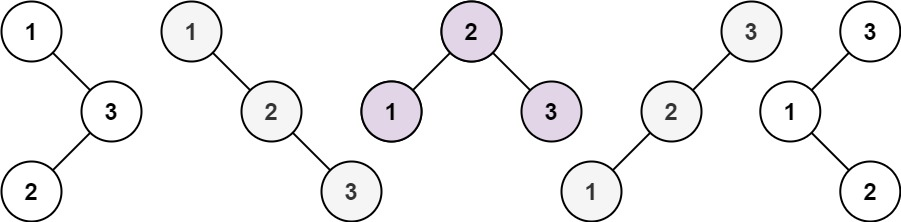
\includegraphics[width=0.65\linewidth]{images/lc0096_eg}
\end{figure}
\item {\colorbox{CodeBackground}{\lstinline|n = 1 --> 1|}}
\end{itemize}

\subsection*{Solution - Recursion}\label{solution:lc0096_recursion}
\begin{lstlisting}
int numTrees(int n) {
  if (n <= 1) { return 1; }
  int cnt = 0;
  for (int i = 0; i < n; ++i) { cnt += numTrees(i) * numTrees(n - (i + 1)); }
  return cnt;
}
\end{lstlisting}

\subsection*{Other Solutions}
\begin{itemize}
%\item \hyperref[solution:lc0096_recursion]{Recursion}
\item \hyperref[solution:lc0096_dp]{DP}
\end{itemize}